\chapter{Related Work and Ideas}

The aim of this chapter is to provide the readers with a holistic view of microservices, design patterns and performance evaluation, especially highlighting some of the important terminology and latest developments in the field. The discussion will consider the existing literature which illustrate how the topics have been previously explored, including the significance of performance engineering for microservices.

\section{Microservices}

Divide and conquer, the idea of breaking down complex systems into smaller manageable parts, is an ancient and proven paradigm which has been applied to computer science since the early 1960s. To tackle the complexities of software systems, concepts such as \textit{modularity} and \textit{information hiding} were introduced in 1972 by D. Parnas \cite{parnas72}, as well as \textit{separation of concerns} by E.W. Dijkstra in 1974 \cite{dijkstra74}.

Regarding the term "microservices", the two most acknowledged definitions were given by Lewis and Fowler \cite{lewis14} and Newman \cite{newman14}, both around the same time in 2014. Newman considers microservices as a particular way of implementing SOA (Service-oriented Architecture) well, whereas Lewis and Fowler define it as a new architectural style contrasted against SOA:

\textit{"In short, the microservice architectural style is an approach to developing a single application as a suite of small services, each running in its own process and communicating with lightweight mechanisms, often an HTTP resource API."}

The aforementioned definitions are first compared in 2016 by Zimmermann \cite{zimmermann16}, who contrasted them with existing SOA principles and patterns. Since then, a number of systematic mapping studies have been published (\cite{pahl16}, \cite{alshuqayran16}, \cite{difrancesco19}) to identify existing literature on microservices, in an effort to bridge the gap between academia (lack of many significant publications) and industry (racing past academia in terms of popularising and adopting
microservices). In particular, Di Francesco et al. \cite{difrancesco19} cite both the prior studies conducted by Pahl and Jamshidi \cite{pahl16} and Alshuqayran et al. \cite{alshuqayran16}, and mention that due to the \textit{bottom-up} approach (practical solutions first) that the industry has taken with microservices, many "fundamental principles and claimed benefits have still to be proven". By learning from practical applications, the industry has identified best practices, however aspects such as performance, functional suitability and maintainability of microservices at the industry-scale (instead of small-scale examples) are yet to proven in academia.

In the past decade or so, the adoption of microservices has been accelerated by the success of companies such as Amazon Web Services (AWS) \footnote{\url{https://aws.amazon.com}}, Netflix \footnote{\url{https://www.netflix.com}}, Spotify \footnote{\url{https://www.spotify.com}} and Uber \footnote{\url{https://www.uber.com/}}. Amazon also has a whitepaper describing how microservices can be implemented using AWS cloud services, taking into consideration ways to reduce operational complexity and design distributed systems components (service discovery, data management, configuration management, asynchronous communication, and monitoring) \cite{aws-microservices}.

\section{Software design patterns}

In software engineering and related fields, \textit{design patterns} are generally defined as reusable solutions to commonly occurring problems in software design. Although design patterns cannot be directly converted to code (like an algorithm described in pseudo-code), they provide a blueprint on how a problem can be approached in various situations. Unlike \textit{algorithms}, design patterns are not meant to define any clear set of instructions to reach a target, but instead provide a high level description of an approach. The characteristic features and final result are laid out, however the actual implementation of the pattern is left up to the requirements of the business problem and use case. Every "useful" design pattern should describe the following aspects: the intent and motivation, the proposed solution, the appropriate scenarios where the solution is applicable, known consequences and possible unknowns, as well as some examples and implementation suggestions.

Over half a decade of software engineering experience has taught developers that it is indeed rare to come across a hurdle that hasn't been crossed before in some shape or form. Most obstacles and day-to-day decisions would have been tackled previously by another developer, thanks to which the idea of \textit{best practices} has been formed over the years. Such solutions are accepted as superior, as they save time, are adequately efficient, and don't have many unknown side effects.

The most widely known literature on the topic is the 1994 textbook \cite{gof94} by the Gamma, Helm, Johnson and Vlissides (Gang of Four), which is considered as the milestone work that initiated the concept of software design patterns. The authors, inspired by Christopher Alexander's definition of patterns in urban design \cite{alexander77}, describe 23 classic patterns that fall under 3 main categories: \textit{creational, structural}, and \textit{behavioral} patterns.

\begin{itemize}
	\item Creational patterns such as \textit{Factory Method, Builder} and \textit{Singleton} increase the flexibility and reusability of code by providing object creation mechanisms.
	\item Structural patterns such as \textit{Adapter, Bridge} and \textit{Facade} illustrate the process of building large, flexible and efficient code structures.
	\item Behavioral patterns such as \textit{Chain of Responsibility, Iterator}, and \textit{Observer} provide guidelines to distribute responsibilities between objects, and are specific to algorithms.
\end{itemize}

In recent times, design patterns have had a tendency of coming across as somewhat controversial, primarily due to a lack of understanding about their purpose. In this regard, it is important for developers to note that in the end, design patterns are merely guidelines and not hard-and-fast rules that must be conformed to.

\section{Common design patterns in microservice architecture}

Several attempts have been made to  apply the concepts of software design patterns to microservices and categorise commonly seen patterns. In Fig. \ref{fig:richardson-patterns}, C. Richardson provides a number of pattern groups, including \textit{Decomposition, Data management, Transactional messaging, Testing, Deployment, Cross-cutting concerns, Communication style, External API, Service discovery, Reliability, Security, Observability} and \textit{UI} \cite{richardson-patterns}.

\begin{figure}[h]
	\centering
	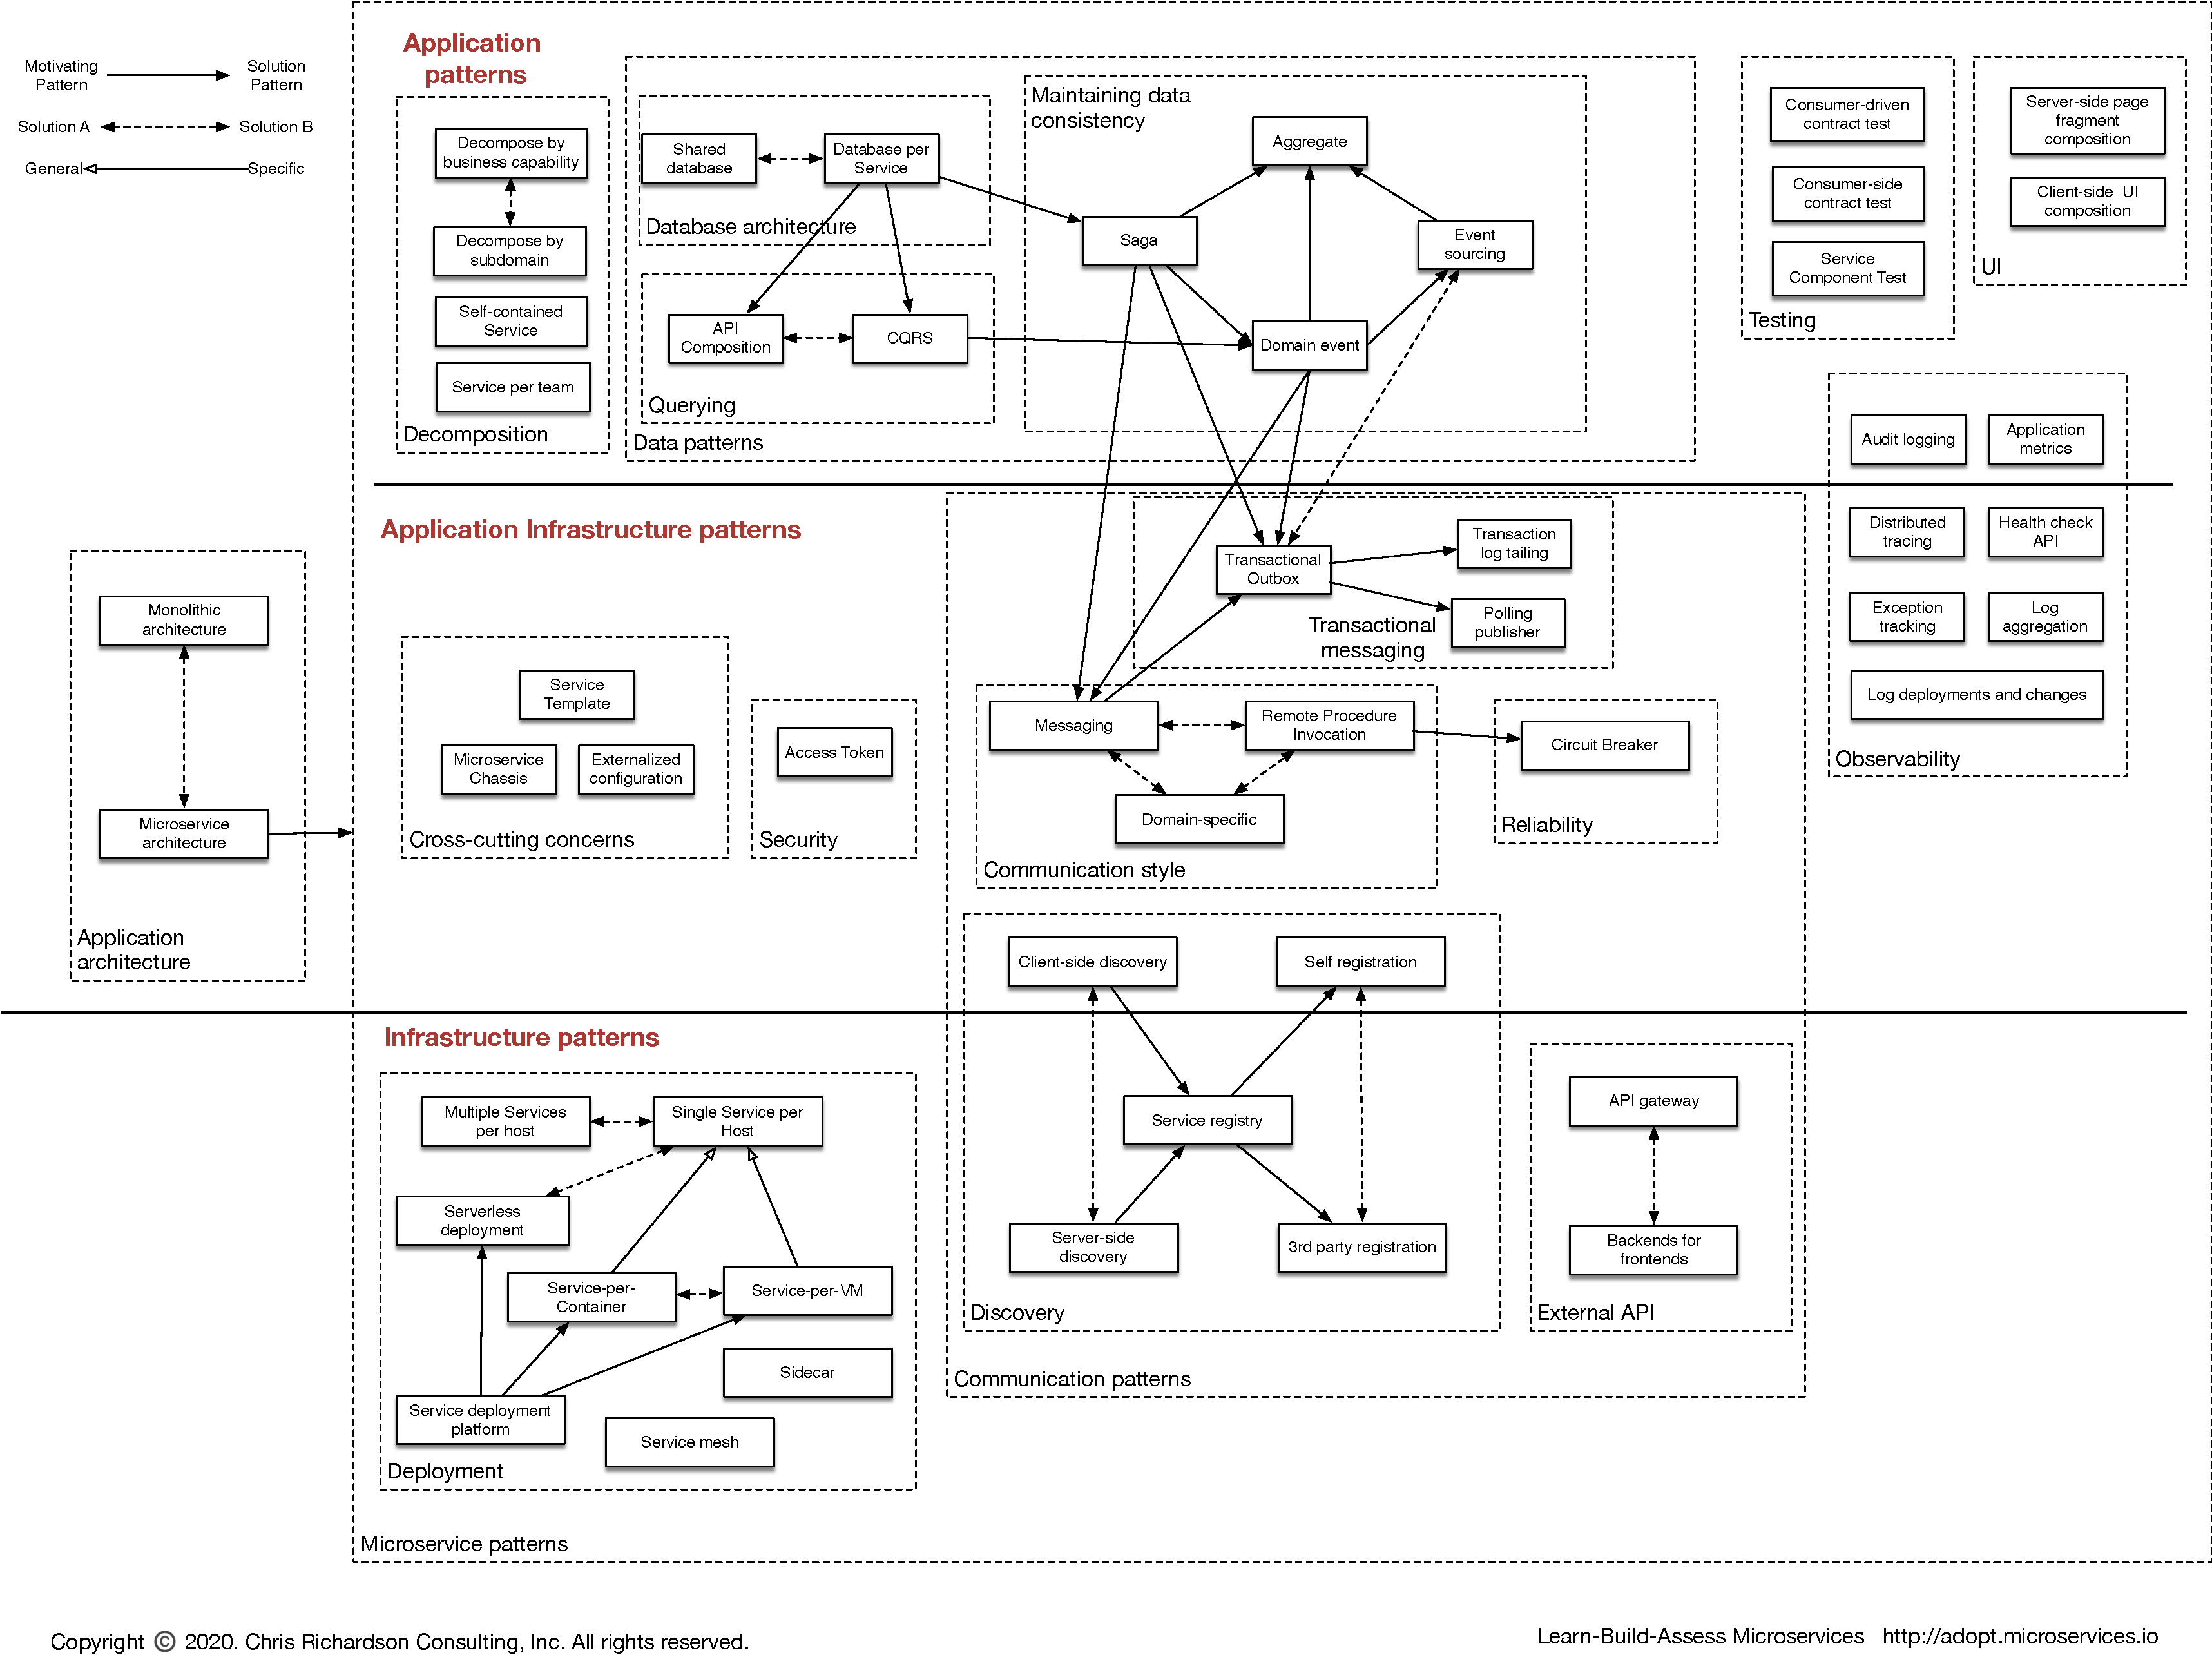
\includegraphics[width=1.0\linewidth]{./assets/images/related-work/richardson-patterns.pdf}
	\caption{Groups of microservice design patterns \cite{richardson-patterns}.}
	\label{fig:richardson-patterns}
\end{figure}

Similarly, M. Udantha describes 5 different classes of design patterns applicable to microservices, namely \textit{Decomposition, Integration, Database, Observability} and \textit{Cross-cutting concerns} (see Fig. \ref{fig:udantha-patterns}).

\begin{figure}[h]
	\centering
	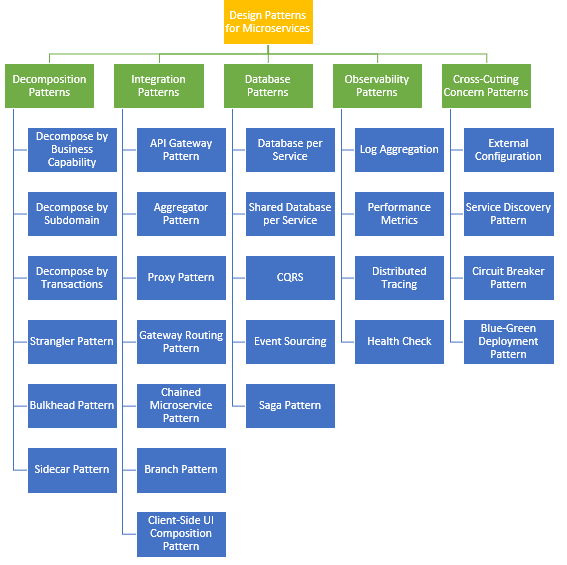
\includegraphics[width=0.6\linewidth]{./assets/images/related-work/udantha-patterns}
	\caption{Udantha's 5 classes of microservice design patterns \cite{udantha19}.}
	\label{fig:udantha-patterns}
\end{figure}

It is important to note that despite minor differences in the categorisation of patterns, the groups suggested by the authors above are generally along the same lines, and aim to address the common principles of microservice design, such as scalability, availability, resiliency, flexibility, independence/autonomy, decentralised governance, failure isolation, auto-provisioning and CI/CD (continuous integration and delivery) \cite{udantha19}.

\begin{itemize}
	\item \textit{Decomposition} patterns lie at the heart of microservice design, and illustrate how an application can be broken down by business capability, subdomain, transactions, developer teams, etc. They also include refactoring patterns that guide the transition from monoliths to microservices.

	\item \textit{Data management} patterns guide the design of database architecture (e.g. whether multiple services will share a database or each service will get a private database). They also lay out methods for maintaining data consistency, dealing with data updates and implementing queries.

	\item \textit{Integration} patterns include API gateways, chain of responsibility, other communication mechanisms (e.g. asynchronous messaging, domain-specific protocols), as well as user interface (UI) patterns.

	\item \textit{Cross-cutting concern} patterns describe ways of dealing with concerns that cannot be made completely independent, and result in a certain level of tangling (dependencies) and scattering (code duplication). Examples include externalising configuration, handling service discovery (client-side such as Netflix Eureka \footnote{\url{https://github.com/Netflix/eureka}}; server-side like AWS ELB \footnote{\url{https://aws.amazon.com/elasticloadbalancing/}}), using circuit breakers, or practising Blue-Green deployment (keeping only one of two identical production environment live at any time). Service discovery and circuit breaker (for reliability) are also considered as communication patterns.

	\item \textit{Deployment} patterns illustrate multiple ways of deploying microservices, including considerations about hosts, virtual machines, containerisation, number of service instances, as well as serverless options.

	\item \textit{Observability} is a part of performance engineering, and such patterns are essential to any form of software design, since application behaviour must be continuously monitored and tested to ensure smooth working. Aggregating logs, keeping track of performance metrics, using distributed tracing, and maintaining a health check API are some invaluable practices which aid the troubleshooting process.
\end{itemize}

It is interesting to note that there are certain similarities between the \textit{GoF}'s creational, structural and behavioral patterns \cite{gof94} and the aforementioned microservice-specific patterns. \linebreak

Apart from the sources mentioned above, there have been some studies conducted to recognise architectural patterns for microservice-based systems. In \cite{bogner18}, Bogner et al. perform a qualitative analysis of SOA (Service-oriented Architecture) patterns in the context of microservices. Out of 118 SOA patterns (sources: \cite{erl09}, \cite{erl12}, \cite{rotem12}), the authors found that 63\% were fully applicable, 25\% were partially applicable and 12\% were not all applicable to
microservices. Taibi et al. \cite{taibi18} tackle the issue of inadequate understanding regarding the adoption of microservice architectures. The authors explore a number of widely adopted design patterns, under the categories of \textit{Orchestration and Coordination, Deployment} and \textit{Data storage}, by elaborating the advantages, disadvantages and lessons learnt from a number of case studies. Thus, a catalogue of patterns is presented, all constituents of which demonstrate the common structural properties of microservices as discussed earlier.

\section{Issues and challenges with microservices}

Although microservice architectures have a number of benefits, it is important to note that they are not universally applicable to solve all problems at scale. Moreover, there are various trade-offs to consider, and \textit{anti-patterns} ("bad practices") to avoid when building new microservice-based systems or transitioning from monolithic applications.

In \cite{cully20}, K. Cully investigates whether unforeseen performance issues can be introduced in a healthy system by independent communication and resiliency configuration of microservices. Using a custom-built rapid prototyping suite, Cully shows that multiple operational constraints in microservices can be conflicting, and optimising the performance within one part of microservice-based system can lead to major pitfalls in other parts.

M. Fowler argues in \cite{fowler14} that transitioning from a well-defined monolith to an ecosystem of microservices has various operational consequences and complexities, which demand certain competencies such as rapid resource provisioning (characteristic of cloud-native applications), observability and monitoring setup, CI/CD, as well as DevOps culture in the organisation. Fowler goes on to elaborate on some of the trade-offs that teams face when choosing microservices over monoliths. The costs associated with microservices include dealing with the distributed nature of the system, with issues such as slow remote calls, risk of failure, consistency, as well the increased operational effort required by teams \cite{fowler15}.

Finally, it is important to avoid common anti-patterns that are known to be counterproductive when adopting the microservice architectural style. A few examples of such practices include \cite{alagarasan15}, \cite{kanjilal21}:

\begin{itemize}
	\item Distributed monolith - a monolith refactored into several smaller services, all of which are interdependent (tightly coupled).
	\item Dependency disorder - services must be deployed in a particular order to work.
	\item Shared database - resource contention due to all microservices sharing a single data store.
	\item API gateway - not using an API gateway, or using it incorrectly by building a gateway in every service.
	\item Entangled data - all services get complete access to all database objects (not following the principle of least privilege).
	\item Improper versioning - services such as APIs not designed for changes and upgrades, leading to reduced maintainability.
\end{itemize}

\section{Performance engineering}

Having discussed the background research and ideas related to microservice-based systems and design patterns, it is now appropriate to narrow down the focus to performance engineering, especially in the context of microservices and their design patterns. Software performance engineering (SPE) is a vital part of the software design lifecycle, including, but not limited to performance simulation and modelling (e.g. using UML \footnote{\url{https://www.uml.org}} diagrams), benchmarking, monitoring, and performance testing.

\subsection{Distributed systems}

Innovation in performance engineering has often been driven by breakthroughs in industry, out of necessity. In fact, Netflix is well known for pioneering the concept of \textit{chaos engineering} as early as 2011, when migrating to the cloud (AWS). To address the inadequacy of available resilience testing, the company invented a suite of tools (known as the "Simian Army" \cite{netflix-chaos}), the most significant of which is Chaos Monkey \footnote{\url{https://netflix.github.io/chaosmonkey/}}.
Chaos engineering tests the performance of a large-scale system when subjected to experimental failure scenarios, especially in production environments. Similarly, there is the principle of ownership at Amazon, where it is the development team's responsibility to handle the entire software lifecycle including operations, performance testing, and monitoring ("you build it, you run it" \cite{ohanlon06}).

Much work has been done over the years on studying performance engineering techniques for distributed systems in general.

\subsection{Evaluation of microservice-based systems}


\section{Summary}

- Mention limitations of the related works
